\chapter{Contexte}
La gestion des ressources numériques est un besoin dans plusieurs secteurs d’activité, répondre à ce besoin est donc un enjeu principal.
\newline

Actuellement, il existe plusieurs outils ou plate-formes qui permettent le traitement des ressources numériques. Mais désormais, il est possible de tout faire (ou presque) dans une seule et même plate-forme appelée DAM (Digital Asset Management).Un DAM propose les outils nécessaires à la gestion des ressources numériques.
\newline

L’intégration d’un gestionnaire de ressources numériques est favorable dans la gestion quotidienne de millions d’assets à travers plusieurs équipes qui ne sont plus limitées par la contrainte géographique sur l’ensemble des canaux de diffusion, pour tous les territoires. Et tout cela dans une seule plate-forme.
\newline

Au-delà des possibilités marchandes que les DAM peuvent offrir, ils accompagnent les entreprises à chaque étape de la transformation digitale de leur marketing.
Et cela pour leur permettre de déployer progressivement un marketing moderne, apportant une solution adaptable à l’écosystème technique de leur marketing.
\newline

Néanmoins, on constate qu’il existe une problématique lié au choix pertinent du DAM adapté et cela parmi une large gamme sur le marché.
\newline

Pour cela il est important de s'intéresser aux moyens qui permettent de faciliter et apporter des éléments pertinents aux futurs clients, dans la sélection d’un DAM. 
\newline

En se basant sur des tableaux comparatifs d’une liste des DAM  via différents sites de comparaisons et différentes recherches, nous proposons une solution à la problématique.Ce mémoire abordera les étapes de création d’un filtre pour le choix d’un DAM dédié au domaine événementiel sportif qui est notre cas d’étude, ce filtre sera la plus-value par rapport aux filtres existant.
\newline

En mettant en place un système de filtres ciblés, cela permet d’avoir la solution la plus adaptée aux besoins des entreprises et leur permet d’atteindre à terme leurs objectifs. 
\newline


\section{Gestion des actifs numériques }

\subsection{Qu’est-ce qu’on entend par gestion des actifs numériques ?}


Le terme « actifs numériques » désigne toutes les ressources numériques utilisées par l’entreprise dans le cadre de ses activités.
\newline

Il s’agit de tous les documents dématérialisés et mis sous formats numériques comme les documents textes, les images, les photos, les sons et les vidéos.
Si dans le domaine privé ces fichiers peuvent aller de quelques centaines à quelques milliers, dans le secteur professionnel, les bibliothèques multimédias peuvent comprendre jusqu’à plusieurs centaines de milliers de fichiers.
\newline

Les ressources, ce sont aussi les compétences qu’ont les acteurs de l’entreprise à tirer parti de toutes les potentialités du numérique pour développer leur modèle d’affaires, leurs activités et leurs offres de valeur.Le    développement    de    ces    compétences numériques  constitue  la  clé  essentielle  permettant  à l’entreprise numérique de se déployer de manière pertinente.
\newline

La gestion des actifs numériques nécessite une solution adaptée à chaque type de fichier. La tâche, particulièrement fastidieuse et chronophage, inclut généralement la prise en charge des documents dès leur arrivée au sein de l’entreprise, leur tri, éventuellement la mise aux formats adéquats, leur classement dans les dossiers dédiés ainsi que leur mise à la disposition des utilisateurs.
\newline

Compte tenu de la multiplicité des opérations et le nombre de documents à traiter, se doter d’un logiciel performant est recommandé.
\newline
\begin{figure}[!!ht]
  \centering
   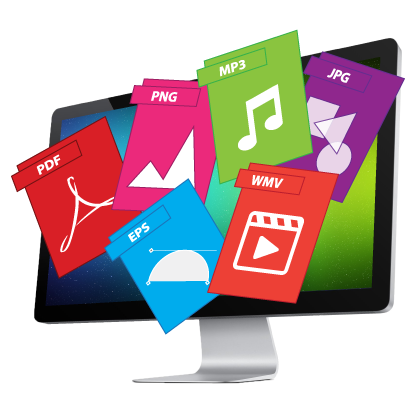
\includegraphics[width=6cm]{introduction/de.png}
  \caption{Gestion des actifs numériques}
  \label{fig:test1}
\end{figure}
 
\newpage
\subsection{Les actifs numériques d'une entreprise}

Pour les entreprises, l’image doit être entretenue c'est d'ailleurs un moyen rapide de se faire connaître et créer un lien avec le consommateur.
\newline

Dans les entreprises du secteur sportif , les photos et vidéos de sport possèdent une puissance émotionnelle incomparable. Aujourd’hui plus que jamais, ces contenus multimédias constituent un vecteur majeur de communication et de promotion des entreprises et des marques sur Internet, auprès de clients cibles et/ou de communautés.
\newline

Par ailleurs, à l’heure du web 2.0, des réseaux sociaux et surtout du mobile, le consommateur connecté éprouve une lassitude croissante pour la publicité en ligne, qu’il juge intrusive.
Face à ce constat, les entreprises se sont mises en quête d’une alternative pour communiquer sur leurs marques. C’est ainsi qu’est né le concept de « marketing de contenu »

\subsection{Marketing de contenu}
Le marketing de contenu, appelé aussi stratégie éditoriale, est une stratégie marketing qui implique la création et diffusion, par une entreprise, de contenu média afin d'acquérir de nouveaux clients, où l’entreprise met en avant une marque non plus à travers la publicité de ses produits, mais à travers des contenus de qualité, pertinents et exclusifs, pour créer une connexion, puis développer la loyauté de l’audience ciblée envers cette marque. 
\newline

Celle-ci construit ainsi sa relation avec le consommateur / le client, communique subtilement sur ses valeurs et renforce sa crédibilité. La proximité, la confiance et l’autorité gagnée par la marque se traduit alors par de meilleures ventes et une clientèle moins volatile.
\newline


Le tableau 1.1 présente une  comparaison entre la publicité en ligne et le marketing de contenu.
\newline
\newline
\newline


\begin {table}[h!]
\begin{center}
\begin{tabular}{|p{6cm}|p{6cm}|}
\hline \centering{Publicité en ligne} &   \centering{Marketing de contenu}  \cr
\hline Intrusive  & Sollicité \\
\hline Lassante &  Utile \\
\hline  Répétitive & Inspiré confiance \\
\hline  Ponctuelle&  Continu \\
\hline
\end{tabular} 
\end{center}
\caption{Publicité en ligne vs Marketing de contenu }
\end{table}

 



\subsection{Les actifs numériques en société  d'événements sportifs }

Les images de sponsoring sportif sont des vecteurs idéaux pour cette nouvelle forme de marketing. Capables de faire vibrer avec passion celui qui les regarde, elles permettent, plus que tout autre contenu, de créer une relation forte et particulière entre une marque et ses clients/prospects.
\newline

Le parfait exemple de ces nouvelles stratégies de communication est celui de la marque Red Bull. 

Sur la page d’accueil du site internet de la marque, aucune publicité sur les boissons énergisantes Red Bull : la communication ne porte que sur des événements sportifs mettant en valeur la marque (Figure 1.2). Cette stratégie a permis à la marque de s’imposer sur un marché tenu par de très grands acteurs (e.g. Coca-Cola, Pepsi,etc.) en créant un univers qui lui est propre, en lien avec sa cible (ados/jeunes adultes).
\newline


\begin{figure}[!ht]
  \centering
   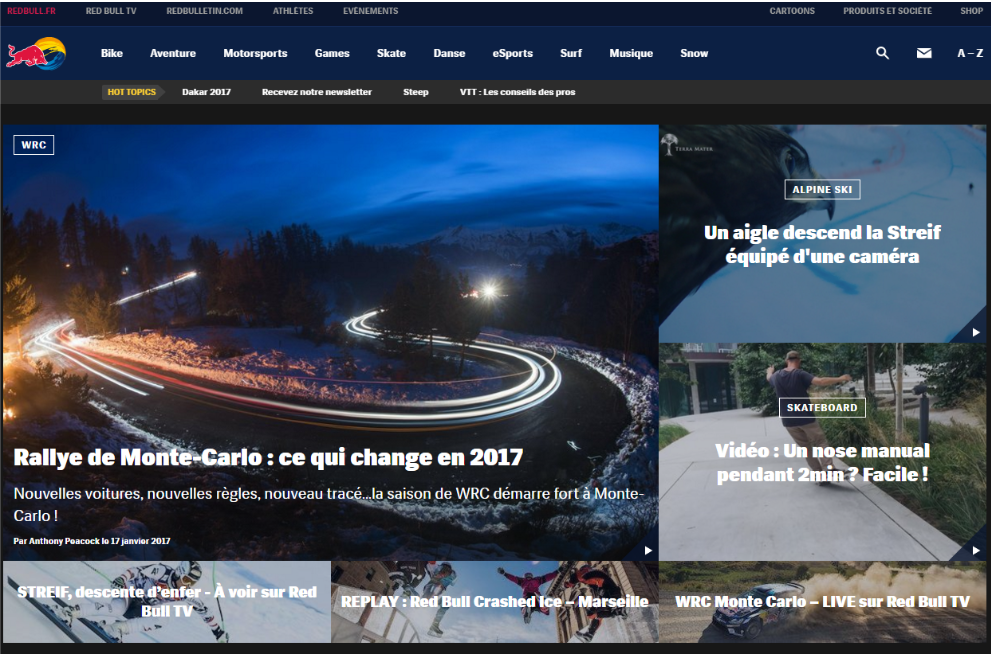
\includegraphics[width=16cm]{introduction/redbull.PNG}
  \caption{Site internet de Red Bull [1]}
  \label{fig:test1}
\end{figure}


Dans ce contexte, l’image et la vidéo deviennent des vecteurs majeurs de communication et de promotion des entreprises et des marques.

\newpage
\section{Outils de gestion de contenus numériques traditionnels}

En général, la gestion des ressources numériques s’opère au moyen d’un logiciel qui facilite le processus.
\newline
De nombreuses entreprises travaillent encore avec des outils et méthodes de gestion de contenus traditionnels comme :


\subsubsection{DropBox}{} 

C’est le service le plus utilisé à ce jour avec plusieurs centaines de millions d’utilisateurs à travers le monde. Dropbox offre 2Gb d’espace gratuits que vous pourrez augmenter un peu en invitant des amis à utiliser le service à leur tour. Photos, vidéos, présentations, documents, fichiers, DropBox garde tout sur des serveurs sécurisés, offre des applications dédiées pour vos appareils mobiles et permet le travail collaboratif en ligne. Pour environ 9 EUR par mois vous accédez à la version pro et un espace de stockage généreux de 1To.
\newline

\subsubsection{WeTransfer}{}

C’est le troisième service sur le podium (google drive et drobox) des services les plus utilisés pour partager des fichiers en ligne. Son succès, WeTransfer le doit à sa facilité d’utilisation et à sa vitesse de téléchargement. WeTransfer dans sa version gratuite ne propose pas de stocker vos documents. Il permet simplement de charger un ou plusieurs fichiers pour les partager avec une ou plusieurs personnes. Vous pouvez charger des fichiers pouvant aller jusqu’a 2 Go. WeTransfer vous proposera soit un lien soit la possibilité d’envoyer directement un mail aux destinataires via la plate-forme.
\newline

Les services de partage et de stockage de fichiers tels que Dropbox et WeTransfer ont connu une croissance explosive ces dernières années, car ils ont tous deux fourni des plates-formes où l'on peut simplement partager et récupérer des fichiers en ligne. Dropbox a donné aux utilisateurs un emplacement central pour stocker tous leurs fichiers et y accéder depuis n'importe quel appareil. Un outil  Digital Asset Managementde (DAM) va encore plus loin et vous donne plus de contrôle sur la façon dont vous gérez vos médias.

\newpage
\section{Les DAM}
\subsection{Définition}{}
Le Digital Asset Management (DAM) est une technologie permettant aux entreprises de stocker, d'organiser, d'enrichir et de partager des ressources numériques de manière intuitive, depuis une source centralisée et sécurisée. 
\newline

Les solutions DAM ont évolué de simples bases de stockage pour ressources numériques à de véritables plates-formes collaboratives, tant pour des entreprises B2B que B2C, impactant différents départements : marketing, équipes créatives, brand management, ventes, et informatiques. 
\newline

La réelle valeur d'une solution DAM réside dans la façon dont vous allez pouvoir exploiter la valeur de vos médias. Stocker des volumes importants de données ne vous coûte rien, et ne vous rapporte rien. Le réel retour sur investissement s'opère dans l'utilisation même des médias, leurs mouvements au sein de votre organisation, que ce soit en interne où via les différentes intégrations à d'autres solutions existantes. C'est là où il est le plus pertinent. 
\newline

\begin{figure}[!ht]
  \centering
   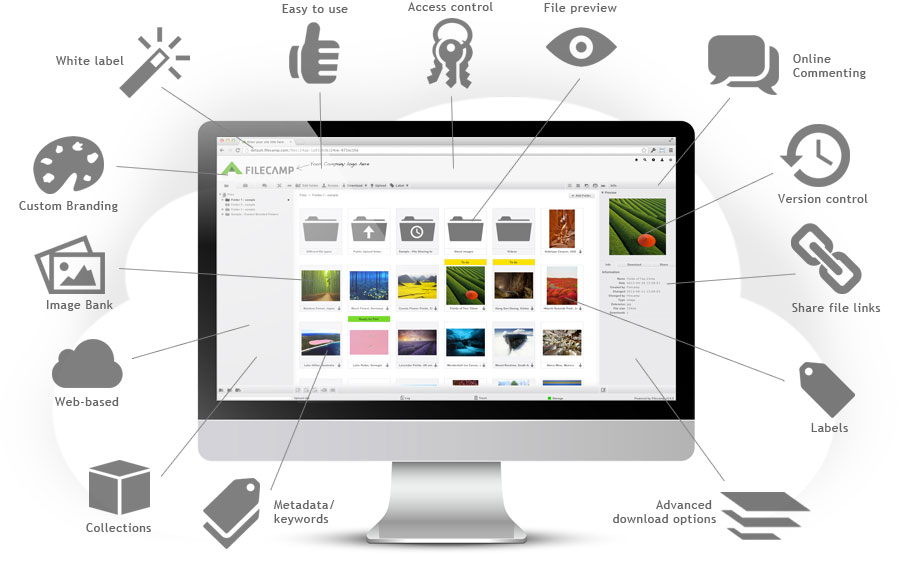
\includegraphics[width=15cm]{introduction/d.png}
   \newline
   \newline
   \newline
  \caption{Digital Asset Management (DAM) [2]}
  \label{fig:test1}      
\end{figure}


\subsection{Est-ce vraiment un DAM?}
Afin de contrer cette question et d'établir une norme, la Fondation DAM (DAMF) a publié les Dix Caractéristiques du DAM. C'est aussi appelé «10 Core».

Les dix principales caractéristiques de la gestion des actifs numériques (DAM) sont les suivantes:
\newline

\begin{enumerate}
\item Les systèmes DAM ingèrent des ressources numériques individuellement ou en masse, et permettent la manipulation de ces ressources numériques
\newline

\item Les DAM sécurisent les ressources numériques qu'ils contiennent avec des listes de contrôle d'accès (ACL) pour les ressources numériques et rôles pour les utilisateurs qui accèdent au système.
 \newline

\item Les DAM stockent les ressource numériques au format binaire, métadonnées et peut stocker plusieurs types de fichiers et permet de personnaliser les champs de métadonnées. 
\newline
 
\item Les DAM permettent de transformer des ressources numériques en de nouvelles formes, telles que des vignettes. Les nouvelles formes générées lors de l'intrusion d'actifs par transformation devraient toutes être stockées en tant que parties de la ressource numérique du fichier original téléchargé.
\newline


\item Les DAM enrichissent les ressources numériques grâce à l'extension des métadonnées et des métriques concernant l'utilisation et la réutilisation de de la ressources numérique tout au long de son cycle de vie.
\newline

\item Les DAM relient les ressources numériques en suivant les relations entre une ressource numérique originale et les versions / variantes de l'originale.
\newline


\item Les DAM régissent un processus structuré dans la gestion, la création et l'évaluation des ressources numériques avec des outils de workflow. Grâce aux flux de travail programmés, les DAM permettent à une main-d'œuvre décentralisée de collaborer ensemble dans un système centralisé.
\newline


\item Les DAM permettent aux utilisateurs de trouver des ressources numériques en facilitant la recherche à travers des métadonnées, des collections.
 \newline


\item Les DAM ont une fonction de prévisualisation qui permet aux utilisateurs de visualiser ou d'ouvrir un fichier sur leur propre appareil avant le téléchargement.
\newline


\item Les DAM produisent / publient du contenu en fournissant des méthodes permettant de partager, d'associer ou de distribuer d'autres éléments en dehors du système. 
 \newline
\end{enumerate}

 
 La Fondation DAM certifie les fournisseurs de DAM qui ont passé le 10 Core et les répertorie publiquement.

D’autres fonctionnalités sont généralement ajoutées par les éditeurs des solutions DAM pour avantager leurs offres.
\subsection{Cycle de vie des actifs numériques}
Comprendre le cycle de vie des actifs numériques est essentiel pour comprendre pourquoi un concentrateur central de gestion de contenu est important. Nous avons identifié quatre phases du cycle de vie des actifs:

\subsubsection{Création}{}La création est bien plus que l'action de filmer une vidéo ou développer des œuvres d'art. La définition des besoins en actifs, la génération d'idées, la planification et le développement font partie du processus créatif.
\subsubsection{Gestion }{}Comprend l'approbation, le contrôle de la version et la logistique permettant aux personnes d'accéder à la visualisation et à l'observation des atouts numériques.
\subsubsection{Distribution}{}  Les groupes internes et externes peuvent faire partie de la distribution. En interne, un actif pourrait se déplacer entre les départements, aux partenaires affiliés ou être acheminé aux vendeurs. 

\subsubsection{Préservation}{}  
Si un actif est stocké pour une utilisation régulière ou est enterré profondément dans les archives, savoir ce que vous avez et accéder à vos actifs est une partie essentielle du cycle de vie des actifs numériques.

    
\begin{figure}[!ht]
  \centering
   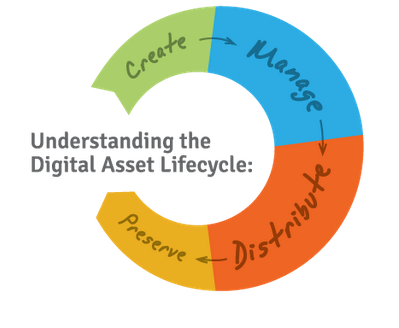
\includegraphics[width=8cm]{introduction/damm.PNG}
  \caption{Cycle de vie des actifs numériques}
  \label{fig:test1}      
\end{figure}


\subsection{Type}{
La nécessité de mieux gérer les actifs numériques a entraîné une plus grande variété d'offres de systèmes DAM. Cette grande variété de programmes de gestion d'actifs numériques pose de sérieux défis à l'acheteur.
\newline

Il existe plus d'une façon de naviguer dans l'océan des DAMs, mais la compréhension des trois modèles de livraison DAM basiques aidera grandement à informer le processus,et c'est une meilleure façon de commencer à réduire votre recherche de fournisseur.

 Il est probable que l'un d'entre eux fonctionne beaucoup mieux pour répondre à des besoins spécifiques de gestion d'actifs numériques que les deux autres. 
 
 
Les modèles de livraison DAM sont:

\subsubsection{SaaS}{}
C’est la gestion d'actifs numériques basée sur le cloud, Il n'y a pas de matériel ou de serveurs à mettre en place chez le client.
Un bon système SaaS DAM est évolutif et peut être consulté n'importe quand par n'importe qui avec une connexion internet.
SaaS est idéal pour une entreprise avec un budget limité pour commencer à utiliser un système DAM prêt à l'emploi.

 \subsubsection{On-permise}{}
Ce système DAM est acheté et installé sur votre matériel, ce qui signifie que vous fournissez l'espace de stockage et les machines pour exécuter l'application.

L'utilisation sur place est fréquente chez les organisations qui ont des besoins de sécurité spécifique pour les informations exclusives. Sur place, vous confiez un contrôle total à votre équipe informatique interne.

  \subsubsection{Open source}{}
Ce système DAM peut être hébergé par un tiers ou sur place. Quoi qu'il en soit, le code source du logiciel est accessible au public.

 Le logiciel open-source est généralement développé de manière publique et collaborative, ce qui peut être un avantage en matière de développement de nouvelles fonctionnalités, mais avec un inconvénient de moins de sécurité.}

\newpage
\section{Les enjeux du DAM }
 
Les marques font face à un enjeu majeur :

Regagner le contrôle total de la gestion, de l’organisation et de la diffusion de leurs contenus et ce, dans un environnement où le marketing digital évolue très rapidement. 
\newline

En fait,le Digital Asset Management n’est pas aussi récent qu’on pourrait le penser: un logiciel similaire existe depuis les 20 dernières années. Or, ces banques d’actifs étaient toujours sur place, complexes à utiliser et nécessitaient de gros investissements.Dans ce monde en évolution constante, accélérée par l’apparition du marketing digital, du mobile et des réseaux sociaux, la quantité des assets et la diversité des formats, que le marketing et la communication doivent produire et gérer, a ainsi explosé.
 \newline
 
Parallèlement, de nombreuses entreprises travaillent encore avec des outils et méthodes de gestion de contenus traditionnels. Ce qui rend donc le travail de centralisation, de recherche et de partage des assets particulièrement difficile. Inévitablement, les solutions de Digital Asset Management historiques ont aujourd’hui une performance, ainsi qu’une efficacité limitée. Cela réduit donc l’autonomie des utilisateurs.
 \newline
 
Avec le Digital Asset Management (DAM), vous pouvez facilement gérer, rechercher, télécharger et partager vos fichiers multimédia directement depuis le web. Toutes vos images, vos films, votre musique, vos logos, vos présentations et vos fichiers PDF sont stockés dans le Cloud, où tous vos collègues du monde entier, à tout moment de la journée.
\newline

  Cependant, certaines solutions DAM ont un grand nombre d’autres fonctionnalités utiles pour gagner du temps, tels que des rapports qui permettent d’obtenir un aperçu des fichiers les plus fréquemment téléchargés et des utilisateurs les plus actifs.
Ainsi, vous pouvez observer les problèmes d’efficacité et améliorer les processus de votre département de marketing encore plus loin. Ils n’étaient pas non plus intuitifs. De nos jours, le digital asset management est entièrement basé sur le Cloud, facile à utiliser et est abordable pour les PME et les multinationales.
\newline

A cause des fonctions comme les “tags” de médias, la recherche de texte, l’importation de médias, les filtres de recherche intelligents etc.., il est facile de trouver le fichier rechercher en quelques secondes seulement. Grâce au système intelligent de distinction des versions, vous pouvez aussi vous assurer que les vieilles versions de modèles ou de logos ne soient jamais diffusés. 

\newpage
\subsection{Différence entre Dropbox et DAM }{}
Les points de différence sont sur les fonctions suivantes :

\subsubsection {1. Recherche et partage des actifs 
}{}


\textbf{Dropbox} permet d'ajouter des noms aux dossiers et aux commentaires sur les fichiers, mais si vous souhaitez effectuer des actions supplémentaires tel le tri ou le filtrage, cela est impossible et quelque soit le type de compte. 

Vous pouvez partager un lien de fichier ou inviter des gens à rejoindre un dossier, mais vous ne pouvez pas choisir ou limiter ce que les gens peuvent faire avec votre contenu (comme l'affichage, le téléchargement ou le partage). Dropbox vous demandera également de mettre à niveau votre compte ou celui de votre destinataire si la taille du fichier dépasse la limite. Le compte gratuit vous offre 2 Go de stockage, ce qui est parfait si vous êtes seul. Mais cela devient très coûteux pour les entreprises avec des centaines de collaborateurs, vendeurs, partenaires et agences qui partagent des centaines d'actifs tous les jours.
\newline


\textbf{Un DAM} a la navigation, la recherche et la prévisualisation intégrées dans au sein de son interface. Vous pouvez rechercher vos biens par type d'actif, métadonnées, statut d'approbation et plus encore. Un DAM vous permet également de rechercher des éléments non textuels comme les fichiers audio, vidéo et image. Lorsque vous téléchargez vos actifs, un DAM peut vous permettre de choisir votre taille de fichier ou votre type de fichier . Cela vous permet de gagner beaucoup de temps et de rendre votre équipe créative satisfaite. De plus, cela vous empêche d'utiliser une application supplémentaire comme Adobe Photoshop pour formater vos images et illustrations.


\subsubsection{2. Back-UPs et suppression des actifs}{}

\textbf{Dropbox} 
\newline
L'un des plus grands défis avec un système de fichiers comme Dropbox est que les fichiers ne sont pas réfléchis ou sauvegardés ailleurs. Cela veut dire que, si vous supprimez un fichier que vous possédez ou que vous avez partagé avec d'autres, il est perdu pour tous les collaborateurs. Beaucoup d'utilisateurs de Dropbox finissent par supprimer des fichiers dont ils n'ont pas besoin d'eux-mêmes, et ne se rendent pas compte que cela supprime les fichiers pour l'ensemble de l'entreprise. Vous pouvez les restaurer dans les 30 jours de la suppression, mais avec des milliers d'actifs à suivre, il est difficile de remarquer lorsque les actifs sont mal placés.
\newline

\textbf{DAM}
\newline
Avec un DAM, vos actifs sont triple-redondants (c'est-à-dire, nous faisons trois copies) et géo-répliqués (tout dans votre DAM est stocké sur 2 sites de serveurs sécurisés différents). Ces mesures garantissent que les actifs peuvent être restaurés facilement et rapidement et vous ne devez jamais vous soucier de supprimer accidentellement un fichier. Avec divers niveaux d'autorisation, les entreprises peuvent restreindre la suppression des actifs à seulement quelques employés sélectionnés, ce qui réduit le risque de suppression de biens précieux.

\subsubsection{3. Niveau de sécurité}{}
\textbf{Dropbox} 
\newline
Dropbox utilise le cryptage SSL pour vos données pendant qu'il se déplace d'un endroit à l'autre et un cryptage sécurisé AES 256 bits pour les données sur le serveur de Dropbox, mais malheureusement, vous ne pouvez pas chiffrer vos fichiers locaux sur votre ordinateur. C'est comme donner à chacun la même clé à votre boîte aux lettres. Avec ce système, toute personne qui se connecte à votre compte Dropbox via votre ordinateur peut accéder à vos fichiers.
\newline

\textbf{DAM}
\newline
Avec un DAM, les normes de sécurité de l'entreprise protègent et chiffrent vos données de bout en bout. Vos atouts numériques sont stockés dans des centres de données sécurisés.

Ce n'est pas un dossier de bureau ou un compte Dropbox où vous videz les fichiers. Et ce n'est pas un lecteur partagé. il faut penser qu'un DAM est un outil de technologie de marketing qui permet de connecter vos actifs numériques à vos clients.
\newline


\section{Le choix d’un DAM} 

Comment choisir une solution de gestion de ressources numériques ?

Dans un contexte où la tendance est à la génération rapide de contenus numériques dans des formats divers et à leur stockage sur différentes plateformes, le DAM constitue un des piliers majeurs de la stratégie de gestion de contenus dans les entreprises. Permettant la maîtrise et la valorisation de son patrimoine et de son image, le DAM vise aussi bien les entreprises BtoB que BtoC, toutes ayant une marque à mettre en évidence.
\newline

Trouver la solution de gestion de ressources numériques qu’il vous faut parmi les nombreux outils DAM (Digital Asset Management) proposés par les professionnels ne sera pas vraiment facile. 
\newline

La meilleure option consiste à définir vos besoins en fonction du type de documents que vous allez traiter d’une part, et de leur nombre d’autre part. Il faut également tenir compte des fonctionnalités qui vous seront utiles (conversion en d’autres formats, fonction indexation, retouches et corrections, etc.). Enfin, il faut considérer la facilité de déploiement de la solution.

Une autre option consiste à choisir une solution polyvalente, notamment si vous utilisez plusieurs types de médias. Cela vous évitera par ailleurs d’avoir à gérer plusieurs outils en même temps. Si vous ne savez pas comment choisir, vous pouvez également vous rendre directement auprès d’un professionnel spécialisé qui vous donnera des conseils avisés et qui saura vous recommander l’outil qui répondra à vos besoins.
\newline

\newpage
Si votre organisation possède un fonds d’actifs numériques à mettre sur le marché, il est recommandé d’associer votre solution DAM à  un outil de gestion commerciale des médias. Ce module complémentaire assure le traitement des commandes effectuées en ligne et le calcul des droits à verser aux auteurs. Il inclut également un système sécurisé pour les paiements via Paypal et des cartes bancaires. L’exportation des données de facturation et de règlement vers les applications comptables peut aussi se faire de manière automatique.


\section{Les avantages des solutions de gestion des actifs numériques}

Un logiciel de gestion des ressources numériques efficace élimine les obstacles et vous aide à vous consacrer entièrement à votre cœur d’activité en vous offrant des outils permettant de transférer, organiser et partager simplement les ressources.\newline

Les solutions de gestion des actifs numériques ont été développées afin de :
\newline

\begin{itemize}
\item   Permettre une grande capacité descriptive avec des métadonnées correspondant  aux différents formats actifs et la possibilité de personnaliser  l’ajout automatique des métadonnées selon les besoins de l’utilisateur.;
\newline
\item  Pouvoir gérer des volumes très importants de contenus numériques.;
\newline
\item    Gérer les droits d’auteurs, licences et toute autre restriction.;
\newline
\item    Pouvoir consulter aisément et rapidement des aperçus d’images;
\newline
\item    Proposer des interfaces intuitives et personnalisables;
\newline
\item    Faciliter la distribution des actifs de l’entreprise;
\newline
 \item   Diminuer les coûts de traitement, de recherche et d’accès aux actifs.
 \newline
\newline
\newline
\newline
\end{itemize} 

\newpage
 \section{La difficulté de gestion des contenus numériques dans les entreprises}

Le Digital Asset Management (DAM) peut être défini comme l’ensemble des technologies, fonctionnalités et opérations permettant la gestion de contenus multimédias par les entreprises. Ceci comprend notamment le sourcing, la sécurisation, l’organisation, le partage, la diffusion et le contrôle desdits contenus. Cette discipline est actuellement en pleine mutation, sous l’impulsion des nouvelles technologies, des nouveaux usages des consommateurs comme des entreprises, et du volume croissant des contenus. La maîtrise du contenu multimédia des entreprises se heurte pour l’heure à 4 principales barrières :

\subsubsection{Fragmentation des contenus des entreprises}{} 
Entre différentes sources, différentes médiathèques,
banques d’images, disques durs des utilisateurs, clés USB, services de stockage comme Dropbox,
Google Drive, systèmes d’administration des sites Internet type WordPress Drupal ou Joomla, etc.,
et le besoin de ces entreprises de centraliser leur patrimoine visuel dans un endroit unique et
sécurisé.

\subsubsection*{La massification des contenus}{} 
 Un volume toujours plus grand de contenus est diffusé chaque jour
sur internet et les réseaux sociaux. Par exemple, 350 millions photos sont postées chaque jour sur
Facebook. 

Ceci posant 2 enjeux pour l’entreprise: l‘obligation d’avoir une infrastructure capable de
supporter le stockage et la diffusion de volumes massifs d’images, car il n’est pas envisageable pour
une entreprise d’avoir son site internet en «panne»; et la nécessité d’avoir des contenus qui se
distinguent des autres, faute de quoi ils demeurent perdus dans la masse. A ceci, le référencement
dans les moteurs de recherches (SEO) est un élément de réponse.
\newline

\subsubsection{Une gestion manuelle chronophage}{}  
 L’ensemble des tâches aboutissant à l’organisation des contenus et leur mise à disposition prend trop de temps, qu’il s’agisse du sourcing des images, de
leur contextualisation, c’est à dire l’ajout d’informations liées à la prise de vue et au sujet de l’image
(géolocalisation, horodatage, métadonnées…), de la gestion des droits d’accès et des droits
d’auteurs, du partage enfin inter ou intra-entreprises dont le process n’est pas optimisé.

Cela abouti
à des bibliothèques de médias mal ou non maintenues, peu ou pas utilisables et délaissées au profit
d’autres sources externes;
\newline

\newpage
\subsubsection{L’absence de contrôle} {}
 une fois diffusé ou téléchargé, l’entreprise perd la maîtrise de son contenu. C’est d’autant plus vrai sur les réseaux sociaux ou les images sont reprises, transmises et
partagées au sein de communautés et par un public devenu acteur (cf. viralité des images).

Parallèlement, les entreprises font face à de nombreuses problématiques:\newline

\begin{itemize}
\item  L’absence d’un modèle de classification universelle des contenus, notamment dans le sport, visant
au développement d’un vocabulaire commun permettant à tous, utilisateurs comme consommateurs,
internes ou externes à une entreprise, de trouver ou retrouver facilement les contenus qu’il cherche
ou veut partager.\newline
\item  La faiblesse de l’indexation des images en tant que contenus dans les moteurs de recherche,
aboutissant à un référencement médiocre privant l’image et son propriétaire de visibilité.\newline
\item  Le manque de collaboration/communication autour des contenus entre les différents membres d’une
organisation (cf. fragmentation, désorganisation, inadaptation, manque de productivité et de
transversalité des outil).\newline
\item  Des usages archaïques comme le téléchargement, reliquat d’une époque pré-digitale, qui empêche la
traçabilité et le contrôle de la diffusion des contenus sur internet et les réseaux sociaux.\newline
\item  La nécessité, pour les entreprises, de diffuser leurs contenus et de communiquer toujours plus vite,
ce qui est irréaliste tant que l’ensemble des tâches antérieures à la publication ou au partage restent
manuelles.
\end{itemize}












